\documentclass[10pt,conference]{IEEEtran}
\IEEEoverridecommandlockouts
% The preceding line is only needed to identify funding in the first footnote. If that is unneeded, please comment it out.
\usepackage{cite}
\usepackage{amsmath,amssymb,amsfonts}
\usepackage{algorithmic}
\usepackage{graphicx}
\usepackage{textcomp}
\usepackage{xcolor}
\usepackage{hyperref}
\usepackage{soul}
\def\BibTeX{{\rm B\kern-.05em{\sc i\kern-.025em b}\kern-.08em
    T\kern-.1667em\lower.7ex\hbox{E}\kern-.125emX}}
\begin{document}

\title{PyTraceBugs: A Large Python Code Dataset \\for Supervised Machine Learning \\in Software Defect Prediction\\
%{\footnotesize \textsuperscript{*}Note: Sub-titles are not captured in Xplore and
%should not be used}
%\thanks{Identify applicable funding agency here. If none, delete this.}
}

\author{\IEEEauthorblockN{Elena~N.~Akimova\IEEEauthorrefmark{1}\IEEEauthorrefmark{2},
Alexander~Yu.~Bersenev\IEEEauthorrefmark{1}\IEEEauthorrefmark{2},
Artem~A.~Deikov\IEEEauthorrefmark{1}\IEEEauthorrefmark{2},
Konstantin~S.~Kobylkin\IEEEauthorrefmark{1}\IEEEauthorrefmark{2},\\
Anton~V.~Konygin\IEEEauthorrefmark{1},
Ilya~P.~Mezentsev\IEEEauthorrefmark{1}\IEEEauthorrefmark{2},
Vladimir~E.~Misilov\IEEEauthorrefmark{1}\IEEEauthorrefmark{2}}
\IEEEauthorblockA{\IEEEauthorrefmark{1} Krasovskii Institute of Mathematics and Mechanics, UB RAS, S.~Kovalevskaya Street 16, 620108 Ekaterinburg, Russia}
\IEEEauthorblockA{\IEEEauthorrefmark{2} Ural Federal University, Mira Street 19, 620002 Ekaterinburg, Russia}
\{aen, kobylkin, konygin\}@imm.uran.ru, \{alexander.bersenev, deykov.artem, ilya.mezentsev, v.e.misilov\}@urfu.ru
}

\maketitle

\begin{abstract}
Contemporary software engineering tools employ deep learning methods to identify bugs and defects in source code. 
Being data-hungry, supervised deep neural network models require large
labeled datasets for their robust and accurate training. In distinction to, say, Java, there is lack of such datasets for Python. 
Most of the known datasets containing the labeled Python source code are of relatively small size. Those datasets are suitable for testing built deep learning models, but not for their training. 
Therefore, larger labeled datasets have to be created based on some well-received algorithmic principles to select relevant source code from the available public codebases.

In this work, a large dataset of the labeled Python source code is created named PyTraceBugs.
It is intended for training, validating, and evaluating large deep learning models to identify a special class of low-level bugs
in source code snippets manifested by throwing error exceptions, reported in standard traceback messages. Here,
a code snippet is assumed to be either a function or a method implementation. The dataset contains 5.7 million 
correct source code snippets and 24 thousands buggy snippets from the Github public repositories. Most represented bugs are: absence of attribute,
empty object, index out of range, and text encoding/decoding errors.

The dataset is split into training, validation and test samples.
Confidence in labeling of the snippets into buggy and correct is about 85\% according to our estimates. 
Labeling of the snippets in the test sample is additionally manually validated to be almost 100\% confident. 

To demonstrate advantages of our dataset, it is used to train a binary classification model for distinguishing 
the buggy and correct source code. This model employs the pretrained BERT-like contextual embeddings.
Its performances are as follows: 
precision on the test set is 96\% for the buggy source code and 61\% for the correct source code
whereas recall is 34\% and 99\% respectively. 
The model performance is also estimated on the known BugsInPy dataset: here, it reports approximately 14\% of buggy snippets.
\end{abstract}

\begin{IEEEkeywords}
defect prediction, bug dataset, data mining
\end{IEEEkeywords}

\section{Introduction}

Identifying deficient source code is a longstanding problem in the software engineering. Bugs in software not only increase development time but can also lead to unexpected program failures, possibly incurring
significant money losses. Numerous software analysis tools are created to assist developers in finding and fixing bugs. These tools can roughly be divided into two groups: static and dynamic analyzers. Static tools try to identify 
bugs in source code without compiling it whereas non-static ones also employ the byte code data. In this work, a bug prediction problem is considered in the Python programs based on their static source code analysis. 
Python has become a language of choice for many developers working in a variety of domains including the web development, data science, and machine learning.
It has its own specifics such as dynamic typing and overwhelming object paradigm in distinction to the other languages such as Java and C\#, which hamper finding bugs.
Moreover, the Python interpreter and existing static analysis tools do not provide any thorough static checks for source code of snippets, postponing revealing of bugs to runtime stage. This leads to the need of debugging
programs, which might be costly. 

Modern static analysis tools and software use a variety of methods including type inference, 
safe refactoring, enforcing coding standards, as well as monitoring specific numeric metrics computed for source code.
Recent advances in machine learning, especially, in deep learning, provide not only a step forward towards improving quality of those methods, but, also,
propose a powerful alternative to them.
For example, some of the existing deep learning models trained on source code~\cite{allamanis2021selfsupervised} employ mining relations between source code entities to be utilized
in bug prediction, localization, and repair. This results in significant improvement over the state-of-the art results.
In the present work, this mainstream line of research is followed to apply deep learning to source code aimed to propose more advanced static analysis tools.

Deep learning models, such as Transformers~\cite{vaswani2017attention} and graph neural networks~\cite{zhou2021graph}, are extremely data-hungry as they have hundreds of millions of parameters to be estimated even during fine-tuning.
There are two ways to collect a large amount of relevant data for training and evaluating these models. The first one is to artificially generate the training and validation samples based on analysis of real source code changes
introduced during bugfixing process. Under this approach, correct source code is corrupted according to some principles of transforming it to buggy, learned from real bugfix changes, made by developers. The corrupted source code 
gives examples of buggy snippets whereas uncorrupted one forms examples of the correct source code  in training and validation samples. Here, the corresponding test dataset is usually a small sized manually
curated dataset of real bugs collected from existing bugfixes stored in version control systems of real projects. 

The main advantage of this approach consists in the fact that an arbitrarily large dataset can be created for training models.
Its drawback is that such a dataset does not reflect actual proportions of bug types in the source code. Moreover, it is confined to some prescribed patterns of corrupting source code to be used to convert correct code into buggy. 
This may result in a certain bias in performance of the bug detectors trained on such datasets.

The second way consists in using real data for
both training and evaluating deep learning models.
Within this approach, both training and validation samples are composed of real examples of buggy and correct source code snippets, automatically collected from available codebases. Here, the data collection process is guided
by some well-understood principles to select relevant source code. To increase confidence of labeling of snippets in the corresponding test sample, it is composed of manually selected snippets analogously to the first approach.

Advantage of this approach is that the model learns from real bugs and works in more or less the same conditions during its training and prediction. As for its drawbacks,
the collected data contain some amount of noise, \textit{e.g.}, either false positives in identifying buggy snippets or false negatives for the correct source code. Here, the proportion must be estimated of such noisy labeling.

In our work, the latter approach is adopted due to the following reasons. The first approach fits best when patterns to corrupt correct source code snippets are more or less 
easy to understand and learn.
This is not the case for other types of simple bugs. 

In the second approach, it is left for models to learn typical patterns of textual difference between buggy and correct snippets from real data. This comes at cost because changes introduced into a buggy snippet are not necessarily confined to 
fixing bugs. They might include refactoring or other changes improving the code quality.

In this work, a PyTraceBugs dataset is created both for training and evaluating of deep learning models for bug prediction
at the granularity of Python functions and methods. More specifically, it is aimed to build predictive models for classical bug prediction problem setting. In this setting, there are two classes
of snippets, which either contain or do not contain bugs. 
The dataset is split into training, validation, and test samples where the test sample is guaranteed to have almost 100\% confident labeling of its snippets.
Moreover, our estimate is 85\% of confidence in labeling of the training and validation samples.

The rest of this paper is structured as follows. Section~\ref{sec2} presents some related work. Section~\ref{sec3} overviews the dataset and describes its content. Section~\ref{sec4} assesses quality of the dataset. Section~\ref{sec5} presents statistics of the code that is included in the dataset. Section~\ref{sec6} describes a bug prediction model trained on our dataset and presents its performance. Section~\ref{sec7} describes in-depth the dataset collection procedures including parallelization.  Finally, we conclude our work in Section~\ref{sec8}.

\section{Related Work}\label{sec2}

In related work, several datasets, which contain buggy source code from a variety of programming languages, are described.
Some of these datasets are intended for developing and evaluating automatic testing and debugging tools. 
They emphasize the features that are valuable for this problem, such as reproducibility of a bug and isolation of a fix. 
The former means that each entity should be accompanied by a test-suite that gives consistent results (failing on the buggy version of code and passing on the fixed one). 
The latter means that the buggy and fixed code should differ only by a bug fix, which does not include irrelevant changes, such as refactoring and adding features.
Most popular datasets of this type for Java and C languages are ManyBugs~\cite{Goues2015manybugs} (185 C bugs) Defects4J~\cite{just2014defects4j} (357 Java bugs), Bugs.jar~\cite{SahaEtAl2018bugsjar} (1,158 Java bugs). 
The BugsInPy dataset~\cite{WidyasariEtAl2020} contains 493 bugs collected from Python projects.

These datasets are usually manually curated, which ensures their high quality. 
However, this type of datasets is not suitable for training machine learning models for defect-related problems 
due to their relatively small size, moreover, reproducibility and isolation are less relevant for static code analysis. 

Larger datasets are usually automatically created. The BugSwarm dataset~\cite{Tomassi2019bugswarm} contains reproducible bugs from open source projects, which are mined from the GitHub platform, using continuous integration services. 
It extracts bug-fix pairs by detecting the code, which fails to build and its subsequent version that passes. 
It contains 1,940 pairs of the Java files and 1,292 pairs of the Python files. 

The common method for automatic collection of large labeled code datasets is to extract data from versioning and bug reporting systems. The main idea is to link reported problems, bugs, and issues with the subsequent code changes to isolate the bugfixing changes and then extract the corresponding buggy and fixed version of the source code.
Most popular algorithm is SZZ~\cite{SZZ2005,Zimmerman2005,Zimmerman2007}. It consists in identifying the bug fixing commit and using the commit message to find the matching issue. However, recent studies~\cite{Mills2018,Herbold2020} show that this approach is prone to mislabeling. Many files found by the basic SZZ algorithm are not the ``pure'' bug fixes. The mistakenly labeled files may contain  changes in the test code, comments, or code refactoring. In our work, special measures are taken to avoid such problems and ensure validity of labeling.

The collected data usually serve multiple purposes.
The first one is the automated program repair. It consists in generating a change that fixes the buggy code (see  survey~\cite{Monperrus2018repair}).
Constructing models for this problem implies analyzing bugs and changes in the dataset to extract and reproduce the patterns that are used to repair the code.

There are several datasets constructed for this task. 
The CodRep dataset~\cite{Chen2018codrep} consists of five parts containing one-line bugfixes from open source Java projects. Its total size is 58,069 commits. 
The work~\cite{Chen2019sequencer} uses this artifact for program repair.

The dataset from~\cite{TufanoEtAl2018} consists of bugfix pairs of Java code mined from the GitHub. 
Its authors identified all commits with messages like ``fix'', ``issue'' or ``bug''. 
For each of such commits, the pair of buggy (precommit) and fixed (postcommit) code fragments is extracted. The resulting dataset contains 800 thousands code pairs.

The ManySStuBs4J dataset~\cite{manysstubs4j} is constructed in the same manner. 
It consists of two parts: 25,539 single-statement (one-line) bugfix pairs from 100 popular open-source Java projects and a larger set of 153,652 pairs from 1,000 projects. 
The authors extracted only those commits, for which both buggy and fixed code passes compilation. 
So, this dataset is confined to simple bugs, which are difficult to spot manually. 
The non-bugfixing changes, such as renaming variables or classes, are excluded. 
The resulting bugfixes form 16 patterns such as variable misuse, wrong function name, wrong operator, \textit{etc}. 

The second application is the software defect prediction. 
Here, the goal is to identify a given code excerpt (file, class, function, or method implementation) as defective or correct (see recent survey in~\cite{Akimova2021survey}).
The defect prediction problem can be posed in different settings. One of the approaches is to consider it as a binary classification problem. Below, are some of the datasets intended to be used in training predictive models for this setting.

The GHPR dataset~\cite{XuWangAi2020} consists of 3,026 pairs of defective and fixed source code files from 307 projects. 
They are extracted from the GitHub by finding pull requests labeled as fixes. 
Then, the resulting code pairs are used to train a graph-based deep learning model for defect prediction.

The BugHunter dataset~\cite{FerencEtAl2020} contains 159 thousands Java bugs with precomputed metrics for three granularity levels (file/class/method). 
It is created from GitHub projects by analyzing the closed and open bug reports containing references to the bugfixing commits. 
The authors use the computed metrics of code to train classifiers for defect prediction.

In the works above, buggy excerpts are distinguished from their instant fixes, \textit{i.e.}, the parts of the bugfix pairs are discriminated from each other.
In our work, a different setting is proposed, which does not treat fixed versions of buggy code as correct.
Namely, it is assumed that a snippet is correct if it is stable, \textit{i.e.}, has not been changed for a significant time period up the current state of software.
This definition of correct source code is more preferable, as guarantees of correctness can not be provided for fix snippets. It is due to the fact that changes can be further introduced into those snippets because of many reasons including fixing other bugs. This idea lies at the core of collecting our dataset.

\section{The PyTraceBugs dataset}\label{sec3}

In this work, a large dataset of Python source code is presented called the PyTraceBugs dataset. This dataset is intended for both training and evaluating
complex (possibly, neural) predictive models for software bug prediction. It is formed by excerpts of source code of functions
and methods from the selected top rated GitHub repositories. It contains examples from both classes
of the correct and buggy source code. 

A range of possible bugs conveyed by the dataset is somewhat restrictive in a sense
that it only contains examples of confirmed bugs. These are the bugs, 
which manifest themselves in the form of raising an error (exception) message, which is called the traceback error message
in Python. This kind of restriction serves two goals. First, this sort of bugs can be considered as low-level, \textit{i.e.}, snippet level. This is the kind of bugs we are aimed to find.
Second, it could simplify the bug localization to some extent as many bugs tend to be near traceback paths
in the graph of function calls. 

Totally, the dataset contains 24 thousands examples of buggy and 5.7 million correct source code snippets from 630 and 10,642 repositories, respectively.
Repositories for the buggy source code employ the standartized GitHub system for handling issues and fixing bugs in their codebase.

In Table \ref{tab2} top 20 most present GitHub repositories are listed accounting approximately 40\% of snippets of buggy code.

\begin{table}[htbp]
\caption{Top repositories per number of buggy snippets}
\begin{center}
\renewcommand{\arraystretch}{1.2}
\begin{tabular}{| l | c | c |}
\hline
  \textbf{Repository name}  & \textbf{Percentage of snippets (\%)}\\
\hline
  saltstack/salt & 7.5\color{lightgray}\%\\
\hline
  ansible/ansible & 5.9\color{lightgray}\%\\
\hline
  Tribler/tribler  & 3\color{lightgray}\% \\
\hline
  pandas-dev/pandas & 3\color{lightgray}\%\\
\hline
  mars-project/mars & 2.6\color{lightgray}\%\\
\hline
  numba/numba &  2.5\color{lightgray}\%\\
\hline
  spyder-ide/spyder &  2.3\color{lightgray}\%\\
\hline
  Cog-Creators/Red-DiscordBot &  1.8\color{lightgray}\%\\
\hline
  pymedusa/Medusa & 1.5\color{lightgray}\%\\
\hline
  python/mypy &  1.4\color{lightgray}\%\\
\hline
  conda/conda &  1.3\color{lightgray}\%\\
\hline
  log2timeline/plaso & 1.3\color{lightgray}\%\\
\hline
  ray-project/ray &  1.1\color{lightgray}\%\\
\hline
  scikit-learn/scikit-learn &  1\color{lightgray}\%\\
\hline
  freqtrade/freqtrade &  1\color{lightgray}\% \\
\hline
  pytroll/satpy  &  1\color{lightgray}\%\\
\hline
   iterative/dvc &  0.9\color{lightgray}\%\\
\hline
  modin-project/modin &  0.9\color{lightgray}\% \\
\hline
  sphinx-doc/sphinx &  0.9\color{lightgray}\%\\
\hline
  scipy/scipy &  0.8\color{lightgray}\% \\
\hline
  Others &  58.3\color{lightgray}\% \\
\hline
\end{tabular}
\label{tab2}
\end{center}
\end{table}

The corresponding distribution of snippets for the correct source code is presented in Table~\ref{tab5}. Here, top 25 repositories account about 15\% of snippets. 
Approximately 16\%  of the repositories of the buggy source code are also present in the correct source code, though, with smaller percentages of snippets.

\subsection{Content of the dataset}

The dataset consists of two parts:
\begin{itemize}
\item automatically collected and filtered source code, containing examples of buggy and correct snippets;

\item a small sample of this automatically collected data, which is
subjected to additional filtering and manual validation by two Python experts.
\end{itemize}

Here, the programmatically collected source code is split into training and validation samples, whereas its manually 
selected sample is used as a test sample. 

The basic principles of automatic selection of examples of correct and deficient 
code snippets from the GitHub repositories for both training and validation samples are given below.
With some specific modifications, they are used in works~\cite{FerencEtAl2020,WidyasariEtAl2020} as a first step to collect datasets of source code
for other programming languages and other research purposes, \textit{e.g.}, for datasets aimed to improve automatic test generation.

Namely, snippets of the correct source code are chosen from stable code of the GitHub repositories
under a simple assumption, which (omitting the details) amounts to the following one:
a snippet is more probably correct if it has not been changed over many commits
up to the latest state of the repository folder it resides in. 

Snippets of source code with bugs are collected from codebase of the top GitHub repositories with issues pages.
More specifically, they are selected from those repositories bugfix commits and pull requests, which are directly related to handling issues marked by bug labels, \textit{e.g.}, named as ``bug'', ``type:bug'' or have any other 
similar label. 

\begin{table}[htbp]
\caption{Top repositories per number of correct snippets}
\begin{center}
\renewcommand{\arraystretch}{1.2}
\begin{tabular}{| l | c |}
\hline
  \textbf{Repository name}  & \textbf{Percentage of snippets (\%)} \\
\hline
  CiscoDevNet/ydk-py & 4.5\color{lightgray}\% \\
\hline
  Azure/azure-sdk-for-python & 1.6\color{lightgray}\% \\
\hline
  oracle/oci-python-sdk  & 0.7\color{lightgray}\% \\
\hline
  sagemath/sage & 0.7\color{lightgray}\% \\
\hline
  cloudera/hue & 0.7\color{lightgray}\% \\
\hline
  tytusdb/tytus & 0.6\color{lightgray}\% \\
\hline
  aliyun/aliyun-openapi-python-sdk  &  0.5\color{lightgray}\% \\
\hline
  home-assistant/core &  0.5\color{lightgray}\% \\
\hline
  cctbx/cctbx\_project &  0.5\color{lightgray}\% \\
\hline
  tencentyun/scf-demo-repo &  0.5\color{lightgray}\% \\
\hline
  Azure/azure-cli-extensions &  0.5\color{lightgray}\% \\
\hline
  sympy/sympy &  0.4\color{lightgray}\% \\
\hline
  dimagi/commcare-hq  &  0.4\color{lightgray}\% \\
\hline
  kovidgoyal/calibre &  0.4\color{lightgray}\% \\
\hline
  docusign/docusign-python-client &  0.3\color{lightgray}\% \\
\hline
  saltstack/salt &  0.3\color{lightgray}\% \\
\hline
  leo-editor/leo-editor  &  0.3\color{lightgray}\% \\
\hline
   tribe29/checkmk &  0.3\color{lightgray}\% \\
\hline
  XX-net/XX-Net  &  0.3\color{lightgray}\% \\
\hline
  {Toontown-Open-Source-Initiative/}& \\{Toontown-School-House}  &  0.3\color{lightgray}\% \\
\hline
  AppScale/gts &  0.3\color{lightgray}\% \\
\hline
  anhstudios/swganh &  0.3\color{lightgray}\% \\
\hline
  SteveDoyle2/pyNastran &  0.3\color{lightgray}\% \\
\hline
  dnanexus/parliament2 &  0.3\color{lightgray}\% \\
\hline
  openhatch/oh-mainline &  0.2\color{lightgray}\% \\
\hline
  Others &  84.8\% \\
\hline
\end{tabular}
\label{tab5}
\end{center}
\end{table}

Besides, only those bugs are considered, which manifest themselves by raising an error exception.
Accordingly, the repositories issues are selected to contain full error traceback reports
on their web pages. These issues report a program crash, which developers consider as a bug and fix it.
Table \ref{tab1} contains error exception types with maximal occurence in the dataset.

\begin{table}[htbp]
\caption{Most common error types in the dataset}
\begin{center}
\renewcommand{\arraystretch}{1.2}
\begin{tabular}{|c|c|}
\hline
  \textbf{Error type}  & \textbf{Percentage of snippets (\%)} \\
\hline
  AttributeError & 16.6\color{lightgray}\% \\
\hline
  TypeError & 15.9\color{lightgray}\% \\
\hline
  ValueError & 10.2\color{lightgray}\% \\
\hline
  KeyError & 8.2\color{lightgray}\% \\
\hline
  RuntimeError & 5.5\color{lightgray}\% \\
\hline
  IndexError &  5.3\color{lightgray}\% \\
\hline
  Others &  38.3\color{lightgray}\% \\
\hline
\end{tabular}
\label{tab1}
\end{center}
\end{table}

The most frequent error messages are the attribute absence, empty object related errors, and index out of bounds error.

\section{Quality of the dataset}\label{sec4}

\subsection{Labeling confidence}

To enforce high confidence of labeling of snippets of the test sample, a manual validation process is conducted to select
relevant snippets from the programmatically collected source code.
Below, ideas are outlined to select examples of the buggy code:
\begin{itemize}
\item a bug reported on the web page of the corresponding issue is simple and easy to understand  (\textit{e.g.}, its actual fix appears near the location where the program crashes, raising an error exception)

\item the reported bug is not dependency, compatibility, or the regression bug;

\item a fix introduced into a buggy snippet is also simple, \textit{e.g.}, is confined to one line;

\item changes (introduced into the snippet) should not be bound to refactoring, \textit{i.e.}, they must be changes fixing the reported bug.
\end{itemize}

These tough restrictions confined 1 out of approximately 15--20 snippets during the validation process. 
The process consisted in reviewing and selecting the buggy snippets among a random sample of several hundreds of the automatically collected entries. 

To filter out the correct snippets with highly confident labeling to be included into the test sample, the following automatic selection principle is used.
Namely, snippets of stable source code are subjected to an additional restriction that
 selects only those snippets, which have many incoming calls from other snippets with many incoming calls. Namely, a graph of calls is computed for snippets of each GitHub repository chosen 
to be a source of stable code for the dataset: snippet 1 is adjacent to snippet 2, if there is a call of snippet 2 in the implementation of snippet 1. A snippet of stable
code is chosen to be included in the test sample, if there are at least 3 snippets with incoming degrees above 3, which are adjacent to that snippet.
In our opinion, this selection criterion must increase visibility of bugs in the source code of selected snippets, and thus, provides additional guarantees that bugs in 
those snippets are more likely to be already revealed and fixed.

The buggy snippets from training and validation samples have more or less confident labeling due to the following specifics of the source code selection from
the GitHub bugfix commits and pull requests:
\begin{enumerate}
\item buggy snippets are being a part of the GitHub bugfixes directly related to issues reporting a program crash in the form of raising an error exception;

\item being selected from the top rated GitHub repositories issues pages, these issues have bug labels; this increases the confidence that the reported problems with repositories source code are bound to be bugs;

\item only highly relevant bugfix commits and pull requests are considered: \textit{i.e.}, they should contain a direct reference to a buggy labeled issue in their message or title and, if it occurs in message, the prescribed tokens should precede this reference \textit{e.g.}, ``closes'', ``fixes'', \textit{etc}.;

\item bugfix commits and pull requests are additionally restricted to handle at most two issues.
\end{enumerate}

To directly estimate quality of the dataset, a percentage is estimated of buggy snippets, for which the corresponding fixes from the bugfix commits and pull requests contain changes, being confined to refactoring.
Such changes are not directly related to bugs. Therefore, the corresponding snippets should be excluded from the collected data as being not correctly labeled.
To obtain a lower bound on the percentage of the refactoring changes present in the training and validation samples,
the rate is estimated for changes from the corresponding bugfix commits, which are bound to docstrings and comments. Namely, it equals to 2.6\%.
Besides, during the manual validation process to form the test sample, our experts observed
approximately 10--15\% of refactoring changes.

To guarantee confidence of labeling of correct source code from training and validation samples, only highly stable source code is selected from the top rated GitHub repositories.
More specifically, a count of commits is computed for each snippet of source code,
which is relative to the directory where this snippet is located. It counts the number of the commits, which contain changes for at least one \textit{.py} file in this specific
directory, but make no changes in that snippet. Only the snippets are selected to be included into training and validation samples, whose corresponding count is above~100.


\subsection{Ability of the cross-project and cross-domain prediction}

The repositories of the training and test samples are made non-overlapping. 
This was done to avoid possible data leaks and provide non-biased performance estimation for models trained on this dataset.
This allows cross-project predictions. 

To explore difference of domains across the training, validation, and test samples, topics are also collected for each repository present in the dataset.
In the GitHub repositories topics are represented by lists of keywords in the main repositories pages.

For the buggy source code, 562 distinct repositories are present in the training sample, whereas 68 repositories are present both in the validation and test samples.
They have 2,345, 424, and 424 distinct topics, respectively. Here, the validation and test samples share the same topics, whereas the  test sample has 228 topics not present in
the training sample.

For the correct source code, 1,571, 10,536, and 94 repositories are present in the training, validation and test samples 
with 3,456, 14,066, and 269 distinct topics, respectively. There are 89 topics in the test sample not present in the validation sample.
Besides, 162 topics of the test sample are not present in the training sample. 

This, to some extent, provides an evidence that
the dataset allows cross-domain predictions.


\section{Summary statistics for the dataset}\label{sec5}

Training and validation samples include 14,089 and 9,457 snippets of the buggy code, as well as, 
351,338 and 5,340,000 snippets of the correct source code respectively. The test sample contains 
170 snippets of the correct source code and 161 snippets of the buggy code.

Table~\ref{tab4} contains statistics for distribution of the buggy code with respect to two its characteristics. The first one is its length in symbols including docstrings and comments.
The second characteristic is the well known cyclomatic complexity, which is a special measure of structural complexity expressed in the form of number of logical paths in source code.
For example, if a snippet does not contain branching statements, \textit{e.g.}, in if-else statements, the cyclomatic complexity is equal to 1; when source code contains a single if-else block statement,
its cyclomatic complexity is equal to 2.

\begin{table}[htbp]
\caption{Statistics of the buggy code}
\begin{center}
\renewcommand{\arraystretch}{1.2}
\begin{tabular}{| l | c | c |}
\hline
  \textbf{Statistic name}  & \textbf{Code length} & \textbf{Cyclomatic complexity}\\
\hline
  Mean & 1,875.9 & 7.0\\
\hline
  Median & 934.5 & 3.0\\
\hline
  Standard error & 3,766.9 & 12.1\\
\hline
  25\% & 426.0 & 1.0\\
\hline
  75\% & 2,010.0 & 8.0\\
\hline
  90\% & 4,081.3 & 16.0\\
\hline
  Min & 19 & 0\\
\hline
  Max &  185,063 & 199 \\
\hline
\end{tabular}
\label{tab4}
\end{center}
\end{table}

Statistics are given in Table~\ref{tab7} for distribution of stable code with respect to its length and cyclomatic complexity.

\begin{table}[htbp]
\caption{Statistics of the stable code}
\begin{center}
\renewcommand{\arraystretch}{1.2}
\begin{tabular}{| l | c | c |}
\hline
  \textbf{Statistic name}  & \textbf{Code length} & \textbf{Cyclomatic complexity} \\
\hline
  Mean & 704.87 & 2.16\\
\hline
  Median & 322.0 & 1.0\\
\hline
  Standard error & 4,089.28 & 5.66 \\
\hline
  25\% & 151.0 & 0.0\\
\hline
  75\% & 734.0 & 2.0\\
\hline
  90\% & 1,596.0 & 6.0 \\
\hline
  Min & 13 & 0\\
\hline
  Max &  6,804,973 & 2,640\\
\hline
\end{tabular}
\label{tab7}
\end{center}
\end{table}

Thus, stable source code is generally shorter and simpler than buggy one.

%\subsection{Topics of the dataset}

Topics of repositories with the buggy code are presented in Table~\ref{tab3}. Here, the snippets can have multiple topics.
Many of the topics are devoted to infrastructure and cloud computing, as well as, to the data science.
Most popular topics for the correct source code are given in Table~\ref{tab6}. A large bulk of topics is devoted to the data science and IOS development.

\begin{table}[htbp]
\caption{Topics of the buggy code}
\begin{center}
\renewcommand{\arraystretch}{1.2}
\begin{tabular}{| l | c |}
\hline
  \textbf{Topic name}  & \textbf{Percentage of snippets (\%)} \\
\hline
  python & 69.6\color{lightgray}\% \\
\hline
  hacktoberfest & 18.6\color{lightgray}\% \\
\hline
  machine-learning  & 12.1\color{lightgray}\% \\
\hline
  cloud & 8.8\color{lightgray}\% \\
\hline
  pandas & 8.5\color{lightgray}\% \\
\hline
  iot  &  7.7\color{lightgray}\% \\
\hline
  infrastructure-as-code &  7.6\color{lightgray}\% \\
\hline
  cloud-management &  7.6\color{lightgray}\%  \\
\hline
  event-management &  7.6\color{lightgray}\%  \\
\hline
  infrastructure-as-a-code &  7.5\color{lightgray}\% \\
\hline
  zeromq &   7.5\color{lightgray}\% \\
\hline
  infrastructure-management  &   7.5\color{lightgray}\% \\
\hline
  cloud-provisioning &   7.5\color{lightgray}\% \\
\hline
  cloud-providers &   7.5\color{lightgray}\% \\
\hline
  infrasructure &   7.5\color{lightgray}\% \\
\hline
  remote-execution  &   7.5\color{lightgray}\% \\
\hline
   infrastructure-automation &   7.5\color{lightgray}\% \\
\hline
  edge &   7.5\color{lightgray}\% \\
\hline
  event-stream &   7.5\color{lightgray}\% \\
\hline
  numpy &   7.5\color{lightgray}\% \\
\hline
  pytorch &  7.3\color{lightgray}\% \\
\hline
  numpy &  6.7\color{lightgray}\% \\
\hline
  data-science &  6.4\color{lightgray}\% \\
\hline
  ansible &  6.2\color{lightgray}\% \\
\hline
  deep-learning &  5.1\color{lightgray}\% \\
\hline
  data-analysis &  4.8\color{lightgray}\% \\
\hline
\end{tabular}
\label{tab3}
\end{center}
\end{table}

\section{Training and evaluating bug prediction models on the dataset}\label{sec6}

Another way to estimate quality of the dataset consists in building predictive models using its data.
Namely, a binary classification problem is considered, in which a given source code
snippet is classified into either buggy or correct. Here, a probability is
estimated for the snippet to contain bugs. The standard logloss is used as a loss criterion, whereas precision and recall
are performance metrics for both validation and test samples. 

In order to apply machine learning models for the considered binary classification problem, feature engineering is first conducted 
 for training, validation, and test samples. In this work, special Transformer-based embeddings are employed for this purpose.
More specifically, the multi-language pretrained CodeBERT model~\cite{FengEtAl2020}\footnote{\url{https://github.com/microsoft/CodeBERT}} is applied.
It uses exactly
the same model architecture as the RoBERTa-base, which includes 12 layers. Each layer has 12 self-attention heads.
Size of each head is 64. The hidden dimension is 768
and inner hidden size of the (pointwise)  feed-forward layer is 3,072.
Total number of model parameters is~125M. 

First, each source code snippet is tokenized using the pretrained CodeBERT tokenizer (which is mostly a standard RoBERTa one). 
It extracts Python keywords, as well as, other words and terms as tokens.
The hidden state of the last layer of the CodeBERT model is computed for each snippet token.
The snippets are fed as input for the model without prelminarily removing docstrings and comments. Maximum model input length is 
512 tokens. Longer source code fragments are truncated to first 512 tokens.

\begin{table}[htbp]
\caption{Topics of the correct code}
\begin{center}
\renewcommand{\arraystretch}{1.2}
\begin{tabular}{| l | c |}
\hline
  \textbf{Topic name}  & \textbf{Percentage of snippets (\%)} \\
\hline
  python & 39.6\color{lightgray}\% \\
\hline
  hacktoberfest & 7.1\color{lightgray}\% \\
\hline
  machine-learning  & 5.2\color{lightgray}\% \\
\hline
  catalyst & 4.5\color{lightgray}\% \\
\hline
  yang & 4.5\color{lightgray}\% \\
\hline
  ydk &   4.5\color{lightgray}\% \\
\hline
   ios-xe &  4.5\color{lightgray}\% \\
\hline
  nx-os &  4.5\color{lightgray}\% \\
\hline
  ios-xr &  4.5\color{lightgray}\% \\
\hline
  deep-learning &  3.9\color{lightgray}\% \\
\hline
  python3 &  2.8\color{lightgray}\% \\
\hline
  pytorch &  2.5\color{lightgray}\% \\
\hline
  science &  2.5\color{lightgray}\% \\
\hline
  django &  2.4\color{lightgray}\% \\
\hline
  tensorflow &  2.2\color{lightgray}\% \\
\hline
  azure  &  2\color{lightgray}\% \\
\hline
   linux &  2\color{lightgray}\% \\
\hline
  data-science &  1.9\color{lightgray}\% \\
\hline
\end{tabular}
\label{tab6}
\end{center}
\end{table}

The hidden state is represented by a vector of 768 numeric features.
Hidden states of tokens are averaged to obtain a final embedding for the snippet. 
Such an embedding is employed as it is a good representation of the snippet tokens and does not lead to information loss.
No further fine-tuning is conducted for the CodeBERT.
 
A LightGBM gradient boosting model is trained on the training sample.
Parameters of the classifier are mostly set to default except the number of iterations and weights for classes. 
Number of iterations is chosen using validation and set to 2,000. To treat imbalance in the training sample,
weights are introduced: for positive (buggy) snippets the corresponding weight is equal to the ratio of the counts of correct and buggy code snippets.

Table~\ref{tab8} presents the experimental results for the test sample of 330 snippets.
Here, precision is 0.96 in the positive class, which means that labeling of the snippets classified as buggy is 96\% confident.
Moreover, among all snippets with bugs, 34\% are labeled as buggy.

Besides, to implicitly check quality of our dataset, the model performance is also estimated on the known manually curated BugsInPy dataset,
which is collected under the principles, similar to those, used to collect our dataset. 
Here, the model correctly selects about 14\% of all buggy snippets. This could be due to the fact that it has been trained to identify only a special
class of bugs, manifested by throwing exceptions, described in traceback reports. In the work \cite{WidyasariEtAl2020}, describing the BugsInPy dataset,
no clear distinction is given of whether the present bugs cause programs throw exceptions.

\begin{table}[htbp]
\caption{Results of the prediction experiments}
\begin{center}
\renewcommand{\arraystretch}{1.2}
\begin{tabular}{| c | c | c | c |}
\hline
    & Precision & Recall &$F_1$-measure \\
\hline
  correct & 0.61 & 0.99 & 0.76 \\
\hline
  buggy & 0.96 & 0.34 & 0.5 \\
\hline
\end{tabular}
\label{tab8}
\end{center}
\end{table}

Two variations of this experiment are also conducted. Namely, the first variation is done using much larger random sample of 1 millon snippets from the correct source code
for the training sample. The second experiment involves another approach to selecting correct source code to be included into the test sample: 90 snippets of the correct
code are randomly chosen to be included into the test sample, such that the corresponding repositories, containing them, are those, which also contain snippets of buggy source code of the test sample;
the rest 80 snippets of the correct source code are chosen randomly. The trained models performance results for both variations are similar to those for the experiment above.

The experiment is also repeated on short source code snippets due to the CodeBERT model restriction for snippets to have at most 512 tokens.
All snippets longer than 512 tokens are removed from the training, validation, and test samples.
For the correct source code, 295,094 snippets are selected out of 351,338 of the training sample, whereas 144 out of 170 fragments are selected for the test sample.
For the buggy source code, 8,537 snippets are chosen out of 14,089 of the training sample, and 83 out of 161 fragments are remained in the test sample.

Table~\ref{tab9} contains the experimental results for the selected subsample of the test sample.
Thus, exclusion of longer snippets disturbs performance metrics up to 0.1.

\begin{table}[htbp]
\caption{Results for the short snippets}
\begin{center}
\renewcommand{\arraystretch}{1.2}
\begin{tabular}{| c | c | c | c |}
\hline
    & Precision & Recall &$F_1$-measure \\
\hline
  correct & 0.7 & 1.0 & 0.82 \\
\hline
  buggy & 1.0 & 0.24 & 0.39 \\
\hline
\end{tabular}
\label{tab9}
\end{center}
\end{table}

An experiment is also conducted where the software metrics are employed. Here, the well known raw, Halstead, and complexity metrics are computed
for the training, validation and test samples using the known Radon library\footnote{\url{https://pypi.org/project/radon/}}. 
All those 22 metrics more or less reflect source code complexity from different points of view. Here, raw complexity amounts to the number of lines of source code,
structural complexity gives the number of operators and operands whereas logical complexity reports the number of different logical paths in the source code.
Computed metrics are combined with the CodeBERT features to produce a predictive LightGBM model. 

Results on the test sample are presented in Table~\ref{tab10}.
Thus, adding software metrics to the CodeBERT features increases $F_1$-measure for the buggy class from 0.5 to 0.7.

\begin{table}[htbp]
\caption{Results for the CodeBERT and metrics}
\begin{center}
\renewcommand{\arraystretch}{1.2}
\begin{tabular}{| c | c | c | c |}
\hline
    & Precision & Recall &$F_1$-measure \\
\hline
  correct & 0.78 & 0.69 & 0.73 \\
\hline
  buggy & 0.71 & 0.8 & 0.75 \\
\hline
\end{tabular}
\label{tab10}
\end{center}
\end{table}


\subsection{Importance of the CodeBERT features for defect prediction}

An experiment is conducted to estimate predictive importance of the CodeBERT embeddings.
Here, the importance is measured using somewhat non-standard method:
it estimates a degree, to which coordinates of the CodeBERT embedding vectors change during the bugfixing process.
Namely, as the buggy snippets in the dataset come from the GitHub bugfixing commits and pull requests, 
each buggy snippet has a pair being a snippet, which represents the most earlier (instant) fix of bugs
in the buggy snippet. 

Thus, to measure importance of the CodeBERT embeddings, one can estimate magnitudes
of differences of coordinates of the CodeBERT embeddings computed both for the buggy snippets and their corresponding paired fix snippets.
In other words, embeddings of two states of the same snippet are compared
right before and after bugfixing changes are introduced in that buggy snippet. 

The adopted method to measure importances is different
from the common one where the importances are measured directly with respect to a given predictive model. 
In our opinion, the former method better reflects sensitivity of embeddings to the bugfixing process as
the fix source code snippet contains changes made to fix only a small number or even a single bug in a short time period. 
In distinction to this,
there can be a long path of bugfixes between a buggy snippet and its stable version. 

To explore distributions of differences between embeddings of the source code before and after bug fixing, all programmatically collected data are used (approximately 24 thousands bugfix pairs).
For each such bugfix pair of snippets, their 768-dimensional CodeBERT embeddings and the corresponding differences are computed. Let them be called ``bug minus fix differences''.
For each component of bug minus fix differences the Wilcoxon signed-rank test is applied and its p-value is computed. 
It tests whether distribution of the bug minus fix differences is symmetric about zero. Then, 
a multiple testing correction (Benjamini--Hochberg) procedure is applied to the list of 768 computed p-values. 
It rejects null hypothesis for 643 out of 768 components of differences vectors at the confidence level of 0.05.
Thus, a vast majority of the CodeBERT features are sensitive to the bugfixing process.

\section{Details of the dataset collection procedure}\label{sec7}

Being most popular source code hosting resource, 
the GitHub is chosen as a source of data for the PyTraceBugs dataset.
An initial list of 150 million GitHub public repositories is first fetched. Among this huge amount, approximately 150 thousands repositories
are selected, whose prevailing language is Python.

Two basic ideas are employed to mine relevant source code.
Namely, to get correct source code snippets, a refined version of the following idea is
used. It is assumed that stable source code from well respected open-source GitHub repositories is more likely to be without bugs. 
As for the buggy source code, it is assumed
that source code of the GitHub bugfix pull requests and commits from the top rated GitHub repositories
is more likely to contain bugs, if those commits and pull requests are linked to
special GitHub issues, having specific labels in repositories issues pages, \textit{e.g}, ``bug'' or ``error''.

There are four levels of decisions made in the dataset collection process:
\begin{itemize}
\item choice of the GitHub repositories to be used as sources of the Python source code;

\item selection of repositories issues to be analyzed for getting the bugfix code;

\item selection of commits and pull requests to be utilized as sources of the bugfix code;

\item choice criteria for the source code snippets to be used to guarantee source code correctness or defectiveness.
\end{itemize}
Below these selection criteria are discussed, first, for the part of the dataset, related to the buggy source code.

\subsection{Collecting source code with bugs}

\subsubsection{Choice of repositories}

To choose relevant repositories, the following principles are employed:
\begin{itemize}
\item issues page is available for a chosen repository;
\item total count of issues is above 18, total count of pull requests is above 17, and the stargazer count is above 50 (these thresholds are 75th percentiles
of counts values)
\item repositories tags or releases count is above 2 (25th percentile) 
\item recent pull requests count over the half a year is above 26 (80th percentile).
\end{itemize}
Repository development in the GitHub is maintained by special web pages where the developers post reports on different issues/problems/bugs
in the repository source code, which are called the issues pages. In well respected repositories, the issues pages are sources of standartized information about bugs in the repositories software,
which allow their automatic processing.

The second selection criterion reflects overall repository popularity and its development activity. Moreover, tags/releases count threshold
filters out those GitHub repositories, whose purpose is not for software development (\textit{e.g.}, for web hosting, learning, or data storage).
The last criterion selects repositories with high recent development activity.

Two first criteria selected about 10,000 repositories, whereas the last one filters about 2,200 repositories among them.
Finally, repositories are filtered by stargazer count above 246 (50th percentile), which finally gives 1,100 repositories.

\subsubsection{Choice of issues}

Besides the issues page, each repository also maintains a labels page, in which a sort of categorization 
of possible types of repository issues is described. The standard practice in the GitHub for marking issues related to reporting bugs in the repository source code
consists in associating these issues with special labels. This standartization allows mining snippets with bugs (see, \textit{e.g.}, \cite{WidyasariEtAl2020,FerencEtAl2020}) by choosing 
only those issues that have a specific label.
Unfortunately, the bug labels names can vary significantly among repositories. Therefore, the final list of criteria to select relevant labels has to be defined
by a set of empiric rules of thumb based on the manual analysis of possible bug labels.

There is also a problem with selection of relevant issues using only bug label. 
Namely, applying this method, it is difficult to single out those issues, which report bugs at the level of snippets (\textit{i.e.}, function or method implementations).
Many repository bugs are at the higher level of library/project functionality.
Since our research focus is on the low-level bugs, some other heuristics must be employed to refine selection of issues.

For the PyTraceBugs dataset, only those issues are selected, whose bug report contains a full error traceback report.
The latter report lists a stack of calls of functions/methods. It ends up with a function or method, in which an error or exception occurs
manifested by the corresponding error message. In our opinion, such issues definitely report low-level bugs. It is because:
\begin{itemize}
\item developers consider such errors/exceptions as bugs by labeling the issue suitably;

\item the actual error occurs at the level of function or method.
\end{itemize}

Moreover, a selection is performed to remove issues, describing certain types of bugs. Namely, the following bugs are discarded: bugs located in dependent libraries
(dependency bugs), bugs related to incompatibility with previous versions of the library (incompatibility bugs), and bugs related to porting parts of newer library version to older version (backport bugs).
This is done based on the issues labels. After applying all selection criteria, 8,165 issues are extracted. 

For the selected repositories and their selected issues, the following information is collected:
\begin{itemize}
\item bug reports (issue titles and labels);

\item full traceback reports and reproducing source code;

\item the commits, pull requests, and merge commits (including their meta information, \textit{e.g.}, titles, messages, states, \textit{etc.}), referenced from issues timelines.
\end{itemize}


\subsubsection{Choice of commits and pull requests}

Source code changes related to handling repository issues are stored in the form of GitHub commits and pull requests.
In addition to those changes, the commits and pull requests contain meta information annotating the made changes, \textit{e.g.}, title, creation or merge timestamp, description,
commit SHA1, pull request URL, \textit{etc}. Among pull requests only merged ones are considered, which contain the code changes finally accepted by developers
to be included into the repositories source code.

In the GitHub, there are several mechanisms of linking commits and pull requests to an issue, which they are aimed to handle.
The information about linked commits and pull requests is available on issues web pages in their sections called the issues timelines.
Four types of commits and pull requests exist:
\begin{itemize}
\item commits/pull requests, which close issues;

\item commits referencing issues;

\item pull requests mentioning issues;

\item linked pull requests.
\end{itemize}
Closing commits and pull requests are highly relevant for the issue they close, \textit{i.e.}, they contain fixes
in the repository source code closely related to handling that issue. Referencing commits are usually also relevant.

There is also a mechanism in the GitHub, which allows one to close an issue when a pull request/commit
is merged/committed. This mechanism prescribes for such commits and pull requests to contain a prescribed keyword and
a reference in their message. This message should refer to the issue that is supposed to be closed, \textit{e.g.}, ``Fixes \#123''. Such commits and pull requests are also relevant.

From the other hand, mentioning and linked pull requests may contain fixes for other issues, which are not directly related to the issue they mention. 
To filter out among such non-closing commits and pull requests, the meta information is used in selecting relevant ones.
Below, our selection criteria are:
\begin{itemize}
\item commit/pull request should not reference more than 2 issues in its message;

\item commit/pull request should contain a reference to issue in its message or title and if it occurs in the message, the prescribed tokens should precede this reference, \textit{e.g.}, ``closes'', ``fixes'', \textit{etc}.
\end{itemize}
When commits/pull requests treat many issues, it is difficult to select only those source code changes, which are relevant for a particular issue.
The first selection rule discards such commits and pull requests. 

In the second selection criterion, the relevance is enforced by providing explicit reference
for issues in commits/pull requests titles or messages, similarly to the standard GitHub mechanism of closing commits/pull requests mentioned above.

Finally, those commits/pull requests are discarded, which contain irrelevant tokens, \textit{e.g.}, ``dependency'' and ``compatibility'' in their titles and messages.
This kind of selection is aimed to remove the code changes related to dependency, compatibility, and backport issues mentioned above.
Applying all the aforementioned selection criteria, 6,013 pull requests and 2,908 commits are selected.

\subsubsection{Choice of the code snippets}\label{h_report_1}


Finally, our selection criteria for the found snippets from bugfix source code are as follows:
\begin{itemize}
\item function/method name does not contain the ``test'' token;

\item full filename for a snippet does not contain the ``test'' token;

\item snippet is syntactically correct.
\end{itemize}

\subsection{Collecting correct source code}

\subsubsection{Choice of repositories}

To select top repositories as sources of the correct source code the following criteria are used: 
\begin{itemize}
\item stargazer count is above 25;

\item forks count is above 25;

\item pull requests count is above 25.
\end{itemize}
As a result of applying those criteria, approximately 11 thousands of repositories are selected.
These criteria are different from the filtering criteria used to get repositories being sources of bugfix source code.
The main difference between them consists roughly in the following. First, in distinction to the criteria described above,
availability of issues pages is also a selection criteria for the bugfix code.
Second, filtering is tighter with respect to the stargazers and recent pull requests counts thresholds. This allows one to get
bugfix source code of more or less high quality from the actively developing repositories.

\subsubsection{Choice of the correct source code snippets}

For correct source code a special type of stable source code is used from the selected repositories.
In general, for top rated repositories, concepts of source code stability and correctness are close.
Namely, developers being mostly highly qualified for such repositories tend to make changes in source code due to many reasons: fixing bugs, adding new features, improve readability and quality, and
treating incompatibility and dependency issues. When the source code becomes of high quality, it becomes stable for a long time period that is specific for
the repository it resides in. Here, there are some exceptions from the rule. For example, abandoned or unused source code tends to be stable.

In this work, the following heuristic is used to filter out relevant stable source code. A count of commits is computed for each snippet of source code,
which is relative to the directory where this snippet is located. More specifically, it counts the number of the commits, which contain changes for at least one \textit{.py} file (its file name does not contain the ``test'' token) in this specific
directory and make no changes in that snippet. Our selection criterion consists in extracting snippets, whose corresponding count is above 100.
This bound allows one to select about 11 million source code snippets (their total size is approximately 650 megabytes).
In addition to this, selected snippets are filtered according to the same criteria as those from the subsubsection \ref{h_report_1}. It gives about 5.7 million snippets.

To form the test sample, 170 snippets are chosen according to the following criterion from the obtained stable source code. A graph of function/method calls is computed within each repository.
For each snippet (denote it by A) two groups of snippets are formed: 
\begin{itemize}
\item the snippets, which call the snippet A in their implementation (these snippets correspond to incoming edges for A in the calls graph);

\item the snippets, which are called from the implementation of A (these correspond to outcoming edges for A).
\end{itemize}
A random sample of 170 snippets is selected from those snippets, for which there are at least 3 incoming edges from other snippets, which themselves have at least 3 incoming edges.
This allows us to protect additionally against the stalled code.

\subsection{Computational cost of collecting the dataset and parallelization}

Collecting the dataset is a time-consuming process because it requires downloading and processing large number of projects from the GitHub platform. 
Besides, the GitHub imposes a limit on frequency of the API requests, which further increases the required time.
Collecting the dataset on a single machine would require about 8 days.
To speed up the process, the Uran cluster \footnote{\url{https://parallel.uran.ru}} is used, which
consists of nodes with two 18-core Intel Xeon Gold 6254 processors. Total list of repositories is split between the computing threads, 
with each of them processing its part of workload. Then, individual results from the threads are combined into a single one. By using 36 threads, the required time reduces to 6 hours.

\section{Conclusion}\label{sec8}

In this work, a large labeled dataset is proposed intended for both training and evaluating of deep learning models
for software bug prediction. It contains a number of examples of real bugs in the Python source code at the granularity of
snippets, \textit{i.e.}, implementations of functions or methods. It is split into training, validation and test samples, containing examples of buggy and correct code snippets.
Confidence in labeling of the snippets in both training and validation samples is about 85\% according to our estimates, whereas it is almost 100\% for the test sample.

To further demonstrate quality of the dataset, a predictive model is built based on it, which classifies snippets into either correct or buggy.
It predicts bugs with precision of 0.96 and recall of 0.34 on the manually validated test sample. 

The dataset is available at \url{https://github.com/acheshkov/pytracebugs}.

%Roughly, there are two types of snippets in the dataset. Snippets of the first type are chosen from stable source 
%code base of most popular GitHub repositories. Snippets of the second type are those excerpts of Python source code, which are revised (corrected) within special
%GitHub commits and pull requests. More precisely, the latter commits and pull requests are referenced from timelines of special GitHub issues,
%being labeled buggy in GitHub repositories issues pages. Such basic ideas to select source code from GitHub lie at the core of many automatic procedures ,
%which are aimed at collecting datasets for defect prediction. 
%Our dataset is collected based on the refined versions of these ideas to improve the dataset quality.

%\begin{table}
%\caption{Table captions should be placed above the
%tables.}\label{tab1}
%\begin{tabular}{|l|l|l|}
%\hline
%Heading level &  Example & Font size and style\\
%\hline
%Title (centered) &  {\Large\bfseries Lecture Notes} & 14 point, bold\\
%1st-level heading &  {\large\bfseries 1 Introduction} & 12 point, bold\\
%2nd-level heading & {\bfseries 2.1 Printing Area} & 10 point, bold\\
%3rd-level heading & {\bfseries Run-in Heading in Bold.} Text follows & 10 point, %bold\\
%4th-level heading & {\itshape Lowest Level Heading.} Text follows & 10 point, %italic\\
%\hline
%\end{tabular}
%\end{table}



%Please try to avoid rasterized images for line-art diagrams and
%schemas. Whenever possible, use vector graphics instead (see
%Fig.~\ref{fig1}).

%\begin{figure}
%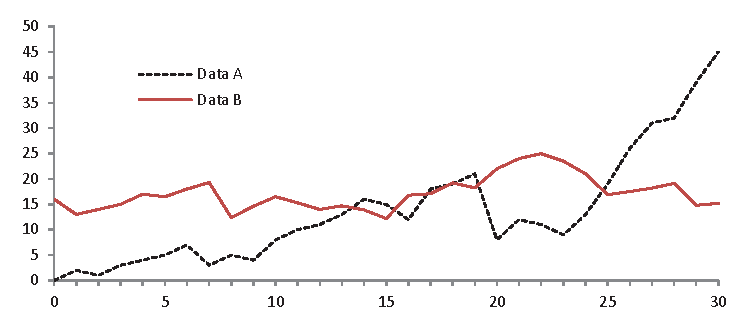
\includegraphics[width=\textwidth]{fig1.eps}
%\caption{A figure caption is always placed below the illustration.
%Please note that short captions are centered, while long ones are
%justified by the macro package automatically.} \label{fig1}
%\end{figure}


%
% ---- Bibliography ----
%
% BibTeX users should specify bibliography style 'splncs04'.
% References will then be sorted and formatted in the correct style.
%

\bibliographystyle{IEEEtran}
\bibliography{references}

\end{document}